% Provenance (never printed): see sources/outline_sources.md (Year 1: physical and chemical
% weathering; hydrolysis and its degrees; the ionic-potential diagram; clay minerals and
% climate; silicate weathering and carbon dioxide). Exercise and problem values in the Book 3
% scratch calculator calc/ch19.py; figure data from figdata/bachelor-1/ionic_potential.py and
% hydrolysis.py. Weathering is owned by Book 1 g5; chemical weathering, hydrolysis, clay mineral
% and laterite by Book 2 g10 (re-founded here). Silicate classes and the feldspars by ch. 7;
% Bowen's series by Book 2 g11; acid--base chemistry, solubility and oxidation by the chemistry
% books; soils and their horizons by the biology books. The silicate-weathering thermostat
% belongs to the Year 2 volume (told).
\chapter{Verwering en kleien}\label{ch:b1:weathering-clays}

De letters van een oude grafsteen vervagen, de scherpe randen van de letters worden afgerond tot ondiepe groeven, sneller op een marmeren steen dan op een leisteen. Een graniet \omterm{def:b1:geological-maps:geological-map}{ontsluiting} die er zo hard uitziet als wat ook op Aarde is, brokkelt aan het oppervlak af tot een korrelig zand, dat tussen de vingers door loopt als losse korrels van glasachtig kwarts, kalkachtig \omterm{def:b1:rock-forming-minerals:groups}{veldspaat} en schilfers \omterm{def:b1:rock-forming-minerals:groups}{mica}. Onder de bossen van de vochtige tropen kan de vaste rots diep liggen, onder een rode aarde die de contouren van de mineralen van de rots bewaart, maar die met een schep kan worden doorgesneden. Alle drie zijn het werk van water aan het oppervlak van de Aarde. Dit hoofdstuk schrijft dat werk uit als scheikunde: welke mineralen het eerst bezwijken, wat zij worden, waarom sommige elementen met het water vertrekken en andere blijven, hoe het klimaat de uitkomst bepaalt, en hoe het trage verval van silicaatgesteente koolstofdioxide uit de lucht trekt.

\begin{recall}
Verwering breekt rotsen af op de plaats waar zij liggen (Boek~1, klas~5). \omterm{def:b1:weathering-clays:weathering}{Chemische verwering} zet de mineralen om; de \omterm{def:b1:weathering-clays:hydrolysis}{hydrolyse} van een \omterm{def:b1:rock-forming-minerals:groups}{veldspaat} geeft een \omterm{def:b1:weathering-clays:clay-mineral}{kleimineraal}, \omterm{def:b1:weathering-clays:clay-mineral}{kaoliniet}, en stuurt kalium en silicium naar de rivieren; een laterite is het rode, ijzer- en aluminiumrijke product van hete, natte klimaten (Boek~2, klas~10). Silicaten worden ingedeeld naar hoe hun \ce{SiO4}-tetraëders hoekpunten delen; een \omterm{def:b1:rock-forming-minerals:silicate-classes}{fyllosilicaat} vormt platen; veldspaten zijn raamwerksilicaten van natrium, kalium en calcium, \omterm{def:b1:rock-forming-minerals:groups}{micas} zijn platensilicaten met kalium tussen de platen (\cref{def:b1:rock-forming-minerals:silicate-classes}, \cref{def:b1:rock-forming-minerals:groups}). De ionstraal van een ion hangt af van zijn lading en van zijn coördinatie (\cref{ch:b1:rock-forming-minerals}). Mineralen kristalliseren uit een afkoelend magma in de volgorde van de reactiereeks van Bowen, \omterm{def:b1:rock-forming-minerals:groups}{olivijn} eerst en kwarts laatst (Boek~2, klas~11). Een zuur geeft waterstofionen af; in water opgelost koolstofdioxide vormt koolzuur; een oxidatie is een verlies van elektronen; een gebalanceerde vergelijking behoudt elk element en de lading (de scheikundeboeken). Een bodem is een levende laag die in horizonten is georganiseerd (de biologieboeken).
\end{recall}

\section{Fysische en chemische verwering}\label{sec:b1:weathering-clays:types}

Een gesteente dat op diepte is gevormd, bij hoge temperatuur en druk en zonder vrij water of zuurstof, is aan het oppervlak uit evenwicht. Het past zich op twee manieren aan, die samenwerken.

\begin{definition}[Fysische verwering, chemische verwering]\label{def:b1:weathering-clays:weathering}
\emph{Fysische verwering}\index{fysische verwering} is het uiteenvallen van een gesteente op zijn plaats in kleinere fragmenten zonder verandering van zijn mineralen. \emph{Chemische verwering}\index{chemische verwering} is de omzetting van de mineralen van een gesteente op zijn plaats door reactie met water en de stoffen die het meevoert, vooral waterstofionen, opgelost koolstofdioxide en zuurstof: sommige mineralen lossen op, andere worden vervangen door nieuwe mineralen die aan het oppervlak stabiel zijn, en een deel van de rots verdwijnt in oplossing.
\end{definition}
% ledger: formoso:weathering

\emph{Vorst.} Water bij \qty{0}{\celsius} heeft de dichtheid \qty{999.87}{kg.m^{-3}}, ijs \qty{916.72}{kg.m^{-3}}: water zet met \qty{9.1}{\percent} uit wanneer het bevriest. Het oude beeld van vorstverwering is
water dat in een afgesloten scheur bevriest en haar openduwt, opnieuw bij elke dooi en vorst. Een model van scheuren in graniet en marmer, gebouwd op de breukmechanica en op wat men over bevriezende gronden weet, legt het gewicht elders: water wordt door de poriën naar ijs in een scheur getrokken, zoals het naar de ijslenzen van een bevriezende grond wordt getrokken, en het ijs groeit en wigt de scheur open zolang de vorst aanhoudt. Aanhoudende vorst is het meest werkzaam tussen ongeveer \qty{-4}{\celsius} en \qty{-15}{\celsius}: dichter bij nul kan het ijs niet genoeg druk opbouwen, en kouder kan het water er niet meer naartoe bewegen.
% ledger: usgs:water-density, iapws:ice-density, wh85:frost

\emph{Verhitting, ontlasting en zout.} Herhaalde verhitting en afkoeling vermoeien een gesteente waarvan de mineralen met verschillende mate uitzetten; een graniet dat door erosie naar het oppervlak is gebracht en van het gewicht erboven is ontlast, zet uit en splijt in platen evenwijdig aan het oppervlak; zouten die kristalliseren uit verdampend water, in woestijnen en aan kusten, wrikken korrels uit elkaar.

\omterm{def:b1:weathering-clays:weathering}{Fysische verwering} doet meer dan gesteente breken: zij opent het voor water.

\begin{proposition}[Het oppervlak dat door versplintering ontstaat]\label{prop:b1:weathering-clays:surface}
Een kubus met zijde $L$, verdeeld in kubusjes met zijde $L/n$, heeft $n$ keer het oppervlak. Algemener heeft een massa $m$ korrels met dichtheid $\rho$, allemaal kubusjes met zijde $d$, het oppervlak $S = 6m/(\rho d)$: het specifieke oppervlak $S/m =
6/(\rho d)$ is omgekeerd evenredig met de korrelgrootte.
\end{proposition}

\begin{proof}
Een kubus met zijde $d$ heeft het oppervlak $6d^2$ en de massa $\rho d^3$, dus het specifieke oppervlak van elke korrel, en van een willekeurig aantal ervan, is $6d^2/(\rho d^3)
= 6/(\rho d)$. Het verdelen van een kubus met zijde $L$ in $n^3$ kubusjes met zijde $L/n$ behoudt de massa en deelt $d$ door $n$, wat het oppervlak met $n$ vermenigvuldigt.
\end{proof}

Een blok \omterm{def:b1:rock-forming-minerals:groups}{veldspaat} met een dichtheid van ongeveer \qty{2600}{kg.m^{-3}} heeft een specifiek oppervlak van \qty{0.23}{m^2.kg^{-1}} als centimeterfragmenten, en \qty{2.3}{m^2.g^{-1}} als micrometerkorrels, tienduizend keer meer. Chemische reacties verlopen aan oppervlakken, dus een gesteente dat door vorst is verbrijzeld of langs zijn voegen is opengemaakt, verweert chemisch veel sneller dan hetzelfde gesteente intact.
% ledger: hom:albite, hom:orthoclase

\emph{De chemische reacties.} Calciet lost volledig op in water dat koolstofdioxide meevoert, waarom marmeren grafstenen hun letters verliezen (Boek~2, klas~10). IJzer(II) van de donkere silicaten wordt geoxideerd tot ijzer(III), dat blijft als geel-bruine en rode oxiden. Het belangrijkst verreweg, omdat silicaten het grootste deel van de \omterm{def:b1:layered-earth:layers}{korst} uitmaken, is \omterm{def:b1:weathering-clays:hydrolysis}{hydrolyse}. De waterstofionen komen van koolstofdioxide, uit de lucht opgelost en door wortels en afbrekers in de bodem uitgeademd, en van de organische zuren van vergaand plantenmateriaal: onbezoedelde oppervlakte- en bodemwateren hebben een pH tussen 5.5 en 7, en het water van de organische laag van sommige bosbodems zo laag als 3.5. Water, temperatuur, oppervlak en zuurgraad zijn zo de vier regelaars van \omterm{def:b1:weathering-clays:weathering}{chemische verwering}, en een warm, nat klimaat met een dikke bodem levert alle vier.
% ledger: formoso:weathering

\section{De hydrolyse van silicaten}\label{sec:b1:weathering-clays:hydrolysis}

\begin{definition}[Hydrolyse van een silicaat]\label{def:b1:weathering-clays:hydrolysis}
De \emph{hydrolyse}\index{hydrolyse (van silicaten)} van een silicaat is zijn reactie met water en waterstofionen, waarbij de waterstofionen de metaalkationen vervangen, die in oplossing gaan; een deel of het geheel van het silicium verlaat de rots als opgelost kiezelzuur \ce{H4SiO4}, en het overige van het \omterm{def:b1:rock-forming-minerals:mineral}{mineraal} wordt opgebouwd tot een nieuw vast stof, een \omterm{def:b1:weathering-clays:clay-mineral}{kleimineraal} of een hydroxide. De oplossing is incongruent: het vaste overblijfsel heeft niet de samenstelling van het aangetaste \omterm{def:b1:rock-forming-minerals:mineral}{mineraal}.
\end{definition}
% ledger: formoso:weathering

Aluminium is de sleutel tot het schrijven van de reactie: bij de pH van bodems en rivieren is het bijna onoplosbaar, en het vaste product houdt het geheel vast. Al het overige volgt daaruit.

\begin{method}[Een hydrolysereactie balanceren]\label{met:b1:weathering-clays:balance}
Gegeven het aangetaste \omterm{def:b1:rock-forming-minerals:mineral}{mineraal} en het vaste product:
\begin{enumerate}
  \item Neem één formule-eenheid van het product, en zoveel van het \omterm{def:b1:rock-forming-minerals:mineral}{mineraal} als er hetzelfde aantal aluminiumatomen bij levert.
  \item Het silicium van het \omterm{def:b1:rock-forming-minerals:mineral}{mineraal} dat het product niet gebruikt, verlaat als \ce{H4SiO4}; de metaalkationen die het product niet gebruikt, verlaten als ionen.
  \item Balanceer de lading van deze kationen met waterstofionen links.
  \item Balanceer de zuurstof met water links.
  \item Controleer het waterstof: het moet vanzelf kloppen. Klopt het niet, dan is een formule fout.
  \item Als een vergelijking met gehele getallen gewenst is, vermenigvuldig alles.
\end{enumerate}
\end{method}

\begin{proposition}[Hydrolyse van de veldspaten]\label{prop:b1:weathering-clays:feldspars}
Met de \omterm{def:b1:weathering-clays:clay-mineral}{smectiet} beidelliet \ce{Na_{0.5}Al2(Si_{3.5}Al_{0.5})O10(OH)2}
(interlaagwater weggelaten), \omterm{def:b1:weathering-clays:clay-mineral}{kaoliniet} \ce{Al2Si2O5(OH)4} en gibbsiet
\ce{Al(OH)3} als producten,
\begin{align*}
&\ce{5 NaAlSi3O8 + 4 H+ + 16 H2O -> 2 Na_{0.5}Al2(Si_{3.5}Al_{0.5})O10(OH)2 + 4 Na+ + 8 H4SiO4},\\ % ce-unbalanced-ok: decimal subscripts the checker cannot read; balance tested in tests/bachelor-1/test_weathering_clays.py
&\ce{2 NaAlSi3O8 + 2 H+ + 9 H2O -> Al2Si2O5(OH)4 + 2 Na+ + 4 H4SiO4},\\
&\ce{NaAlSi3O8 + H+ + 7 H2O -> Al(OH)3 + Na+ + 3 H4SiO4},\\
&\ce{CaAl2Si2O8 + 2 H+ + H2O -> Al2Si2O5(OH)4 + Ca^2+}.
\end{align*}
De albiet verliest \qty{80}{\percent} van zijn natrium en $8/15$ van zijn silicium aan de oplossing in de eerste reactie, al zijn natrium en $2/3$ van zijn silicium in de tweede, al beide in de derde. Het anorthiet verliest al zijn calcium en geen van zijn silicium.
\end{proposition}
% ledger: webmineral:clays-b19, hom:albite, hom:anorthite

\begin{proof}
Pas de methode toe. Eerste reactie: twee beidelliet-eenheden bevatten $2\times2.5 = 5$
aluminium, het aluminium van 5 albiet; de 15 silicium van de albiet min de
$2\times3.5 = 7$ van het product laten 8 \ce{H4SiO4} over; de 5 natrium min 1 laten
4 \ce{Na+} over, in balans met 4 \ce{H+}; zuurstof, $40 + w$ links en $24 + 32 =
56$ rechts, geeft $w = 16$; waterstof, $4 + 32 = 36$ en $4 + 32 = 36$,
klopt. Tweede: 2 albiet geven het 2 aluminium van \omterm{def:b1:weathering-clays:clay-mineral}{kaoliniet}, $6 - 2 = 4$
\ce{H4SiO4}, 2 \ce{Na+} en 2 \ce{H+}; zuurstof $16 + w = 9 + 16$ geeft $w = 9$;
waterstof $2 + 18 = 20 = 4 + 16$. Derde: één albiet, drie kiezelzuren, één
\ce{Na+} en één \ce{H+}; zuurstof $8 + w = 3 + 12$ geeft $w = 7$; waterstof
$1 + 14 = 15 = 3 + 12$. Vierde: het 2 aluminium en 2 silicium van anorthiet zijn
precies die van \omterm{def:b1:weathering-clays:clay-mineral}{kaoliniet}, geen kiezelzuur verlaat, \ce{Ca^2+} heeft 2 \ce{H+} nodig;
zuurstof $8 + w = 9$ geeft $w = 1$; waterstof $2 + 2 = 4$. De geëxporteerde fracties
zijn de ionen in oplossing gedeeld door de atomen in het \omterm{def:b1:rock-forming-minerals:mineral}{mineraal}: $4/5$ en $8/15$, dan
$2/2$ en $4/6$, dan $1/1$ en $3/3$.
\end{proof}

Dezelfde albiet kan dus drie verschillende vaste stoffen geven, en welke het geeft, hangt af van hoeveel water door de rots gaat en de producten wegvoert: weinig water, en veel van het kiezelzuur en enkele kationen blijven achter om een \omterm{def:b1:weathering-clays:clay-mineral}{smectiet} op te bouwen; meer, en alleen genoeg kiezelzuur voor \omterm{def:b1:weathering-clays:clay-mineral}{kaoliniet} blijft; veel, en het kiezelzuur verdwijnt volledig.

\begin{definition}[Bisiallitisatie, monosiallitisatie, allitisatie]\label{def:b1:weathering-clays:hydrolysis-degree}
De graad van de \omterm{def:b1:weathering-clays:hydrolysis}{hydrolyse} van silicaten wordt genoemd naar zijn product. \emph{Bisiallitisatie}\index{bisiallitisatie} vormt 2:1-kleimineralen, zoals \omterm{def:b1:weathering-clays:clay-mineral}{smectieten}, met ongeveer twee siliciumatomen per aluminium; een deel van de kationen blijft erin. \emph{Monosiallitisatie}\index{monosiallitisatie} vormt 1:1-kleimineralen, \omterm{def:b1:weathering-clays:clay-mineral}{kaoliniet}, met één silicium per aluminium; alle alkali- en aardalkalikationen verlaten. \emph{Allitisatie}\index{allitisatie} verwijdert het silicium volledig en laat aluminiumhydroxide achter, gibbsiet.
\end{definition}
% ledger: pedron:stages, formoso:weathering

De bereikte graad is in de eerste plaats een kwestie van klimaat, door de regen en de temperatuur, en daarna van de drainage van het profiel. Waar het water weinig wordt ververst, verliest een graniet veel van zijn natrium en calcium, kalium langzamer, en slechts een deel van zijn silica: zijn veldspaten worden 2:1-kleien, en veel kwarts blijft over; de rots valt uiteen tot een zand van kwarts, \omterm{def:b1:rock-forming-minerals:groups}{mica} en half verweerd \omterm{def:b1:rock-forming-minerals:groups}{veldspaat}, vermengd met klei. Onder de zware regens van de vochtige tropen, meer dan \qty{2000}{mm} per jaar, worden de kationen en het silicium veel meer uitgeloogd, en vormt zich \omterm{def:b1:weathering-clays:clay-mineral}{kaoliniet}, Si/Al = 1. Waar het uitlogen het sterkst is, verdwijnt zelfs het silicium van \omterm{def:b1:weathering-clays:clay-mineral}{kaoliniet}, en blijft gibbsiet over.
% ledger: pedron:stages, goldich:1938, formoso:laterite

\begin{omfigure}
\begin{tikzpicture}[font=\small]
% fractions of albite's Na and Si exported by the three degrees (figdata/bachelor-1/hydrolysis.py)
\begin{axis}[width=10.5cm, height=6cm, ybar, bar width=0.5cm, ymin=0, ymax=112,
    xmin=0.45, xmax=3.55, xtick={1,2,3},
    xticklabels={{bisiallitisatie\\ tot beidelliet\\ (Si/Al = 1.4)}, {monosiallitisatie\\ tot kaoliniet\\ (Si/Al = 1)}, {allitisatie\\ tot gibbsiet\\ (Si/Al = 0)}},
    xticklabel style={align=center, font=\footnotesize},
    ylabel={uitgevoerd in oplossing (\si{\percent})}, ytick={0,20,...,100},
    legend style={at={(0.5,1.03)}, anchor=south, font=\footnotesize, legend columns=2, draw=none},
    nodes near coords={\pgfmathprintnumber[fixed,precision=0]{\pgfplotspointmeta}}, every node near coord/.append style={font=\scriptsize},
    enlarge x limits=false]
  \addplot[fill=omThm!60, draw=omThm!80!black] table[x=degree, y=Na] {figdata/out/bachelor-1-hydrolysis-degrees.dat};
  \addplot[fill=omDef!55, draw=omDef!80!black] table[x=degree, y=Si] {figdata/out/bachelor-1-hydrolysis-degrees.dat};
  \legend{natrium, silicium}
\end{axis}
\end{tikzpicture}

{\small De drie graden van \omterm{def:b1:weathering-clays:hydrolysis}{hydrolyse} van albiet: het percentage van zijn natrium en van zijn silicium dat in oplossing wordt meegevoerd, berekend uit de gebalanceerde reacties, en de verhouding silicium tot aluminium van het overgebleven vaste stof. Het aluminium blijft in alle drie geheel in het vaste stof.}
\label{fig:b1:weathering-clays:degrees}
\end{omfigure}


\begin{omfigure}
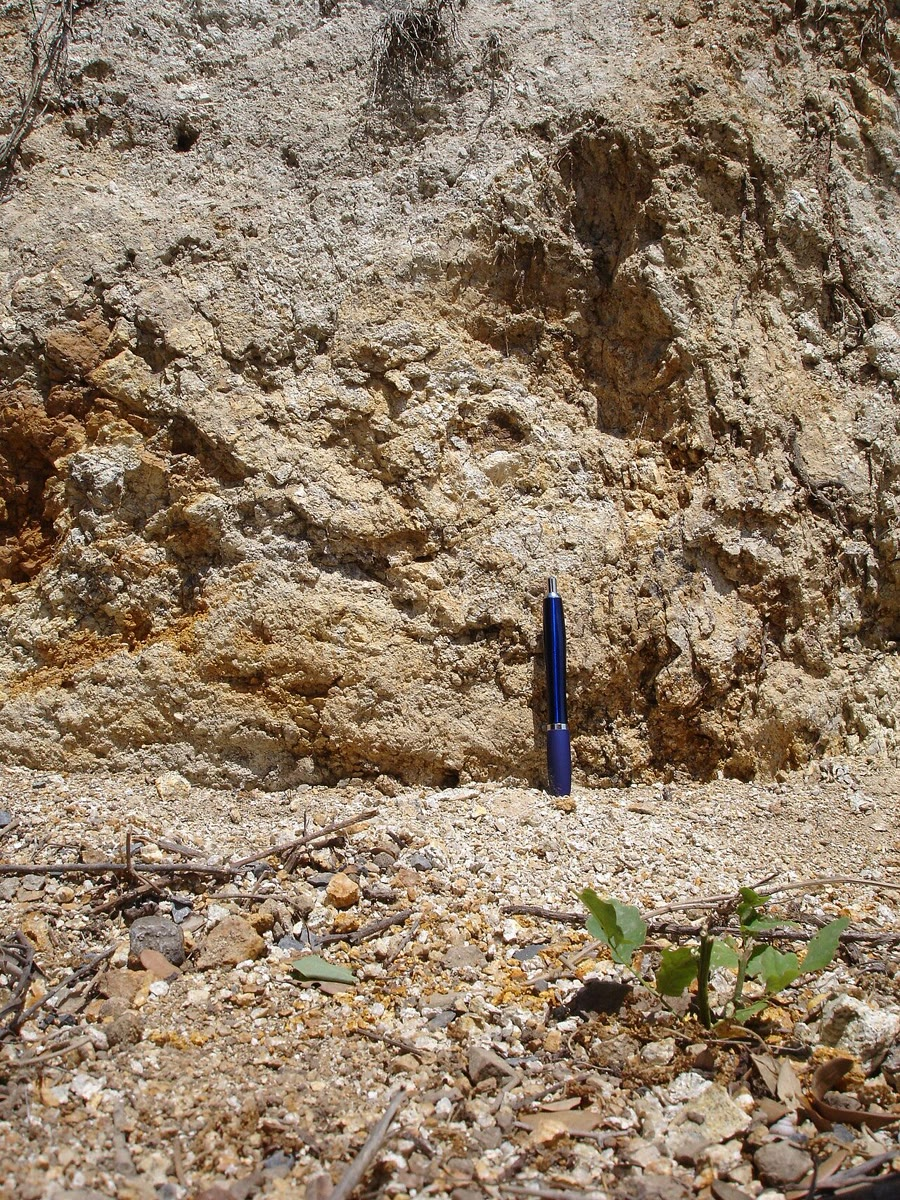
\includegraphics[height=6.3cm]{images/book3/b1-granite-grus.jpg}\hfill
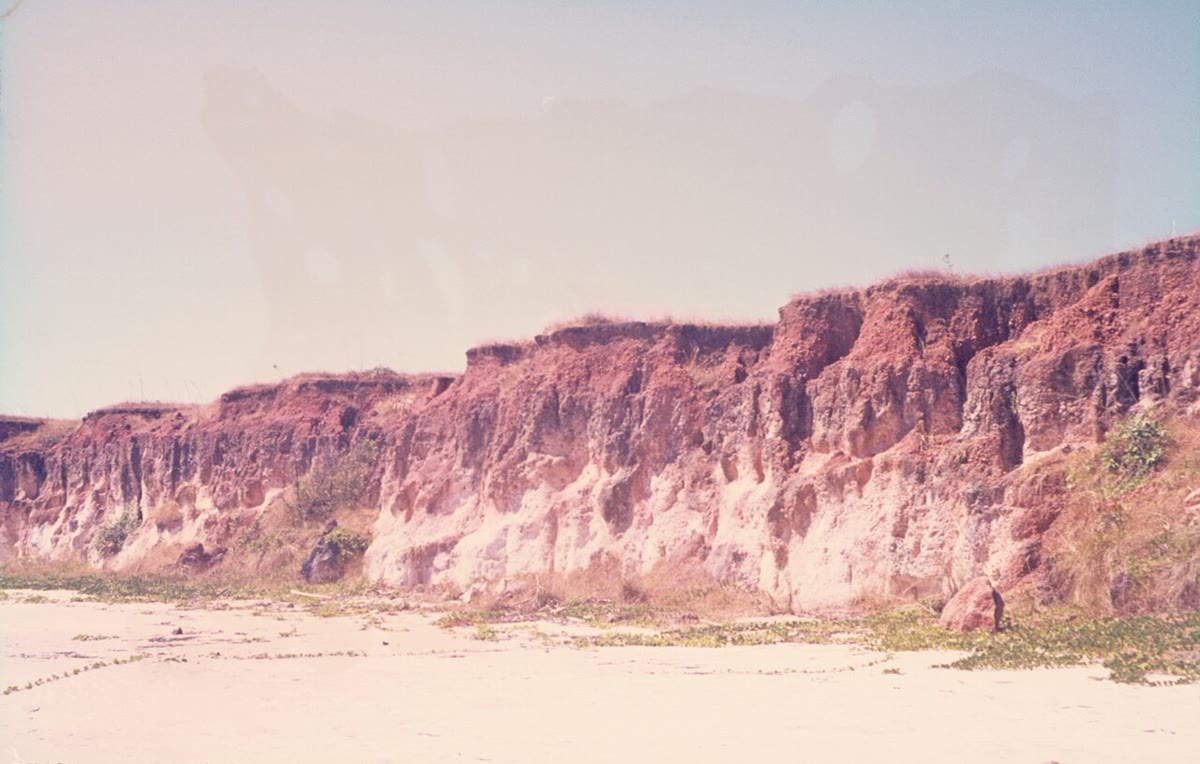
\includegraphics[height=6.3cm]{images/book3/b1-bauxite-weipa.jpg}
\par\smallskip{\small Links: verrotte graniet in de Pyreneeën, nog op zijn plaats maar afbrokkelend tot een zand van kwarts, \omterm{def:b1:rock-forming-minerals:groups}{veldspaat} en \omterm{def:b1:rock-forming-minerals:groups}{mica}, met het losse zand aan de voet; de pen geeft de schaal. Foto: Pinpin, CC~BY~2.5. Rechts: een verweringsprofiel aan de kust bij Weipa, in het noorden van Australië: rode bauxiet, het product van \omterm{def:b1:weathering-clays:hydrolysis-degree}{allitisatie}, boven een witte, kaolinietrijke zandsteen. Foto: Werner Schellmann, 1969, CC~BY-SA~2.5. Beide van Wikimedia Commons.}
\label{fig:b1:weathering-clays:photos}
\end{omfigure}
% ledger: commons:grus, commons:weipa

\emph{Welke mineralen het eerst gaan.} In 1938 vergeleek Samuel Goldich verweerde profielen met hun moedergesteenten, stelde een reeks voor van de mineralen van het minst tot het meest stabiel bij verwering, en vond dat die de volgorde volgt waarin zij uit een magma kristalliseren: \omterm{def:b1:rock-forming-minerals:groups}{olivijn} en calciumrijk \omterm{def:b1:rock-forming-minerals:groups}{plagioklaas} eerst, kwarts laatst. De mineralen die bij de hoogste temperaturen zijn gevormd, liggen het verst van het evenwicht aan het oppervlak. Een moderne lijst, van het minst naar het meest bestendig, luidt: pyriet, calciet, dolomiet, \omterm{def:b1:rock-forming-minerals:groups}{olivijn}, calciumplagioklaas, pyroxenen, intermediair \omterm{def:b1:rock-forming-minerals:groups}{plagioklaas}, amfibolen, biotiet, \omterm{def:b1:rock-forming-minerals:groups}{kalium-veldspaat}, muscoviet, \omterm{def:b1:weathering-clays:clay-mineral}{smectiet}, kwarts, \omterm{def:b1:weathering-clays:clay-mineral}{kaoliniet}, en de oxiden gibbsiet en hematiet. Laboratoriummetingen van oplossingssnelheden bevestigen de rangschikking; het blijft een rangschikking, geen wet, omdat de snelheid van elk \omterm{def:b1:rock-forming-minerals:mineral}{mineraal} ook van het water eromheen afhangt. De eindproducten van verwering, \omterm{def:b1:weathering-clays:clay-mineral}{kaoliniet}, gibbsiet en hematiet, zijn het meest bestendig van alle: zij zijn al stabiel aan het oppervlak.
% ledger: goldich:1938, formoso:weatherability, lasaga:1984

\emph{De massabalans van een verweringsprofiel.} Verwering verwijdert materie, dus een concentratie die in een verweerde rots is gemeten, vertelt niet hoeveel er verloren is: het verlies van andere elementen concentreert die welke blijven. Een element dat niet beweegt, geeft het referentiepunt.

\begin{proposition}[Massabalans met een onbeweeglijk element]\label{prop:b1:weathering-clays:immobile}
Laat $i$ een element zijn dat verwering niet verplaatst, met massafracties $C_{i,p}$ in het moedergesteente en $C_{i,w}$ in het verweerde gesteente. Dan wordt een massa $m_p$ moedergesteente de massa $m_w = m_p C_{i,p}/C_{i,w}$ verweerd gesteente, en is de fractie van elk ander element $j$ die verloren gaat
\[
  f_j = 1 - \frac{C_{j,w}}{C_{j,p}}\,\frac{C_{i,p}}{C_{i,w}} .
\]
\end{proposition}

\begin{proof}
De massa van $i$ blijft behouden: $m_p C_{i,p} = m_w C_{i,w}$, wat $m_w$ geeft. De massa van $j$ gaat van $m_p C_{j,p}$ naar $m_w C_{j,w}$, een fractie $m_w C_{j,w}/(m_p C_{j,p}) = (C_{j,w}/C_{j,p})(C_{i,p}/C_{i,w})$ ervan blijft over; $f_j$ is één min deze fractie.
\end{proof}

Titaan en zirkonium zijn de gebruikelijke keuzes, om een reden die de volgende paragraaf geeft.

\section{Welke elementen vertrekken: de ionische potentiaal}\label{sec:b1:weathering-clays:ionic}

Natrium, kalium en calcium vertrekken met het water; aluminium, ijzer(III) en titaan blijven; silicium zit er tussenin. Het verschil ligt in hoe elk ion zich in water gedraagt.

\begin{definition}[Ionische potentiaal]\label{def:b1:weathering-clays:ionic-potential}
De \emph{ionische potentiaal}\index{ionische potentiaal} van een ion is de verhouding $z/r$ van zijn ladingsgetal $z$ tot zijn ionstraal $r$, hier in ångström (voor dezelfde coördinatie voor alle ionen, zesvoudig in wat volgt).
\end{definition}
% ledger: nomad:goldschmidt, dangic:goldschmidt, shannon:radii-b19

\begin{proposition}[De drie velden van de ionische potentiaal]\label{prop:b1:weathering-clays:fields}
In het water van verwering blijven ionen met $z/r < 3$ in oplossing als gehydrateerde kationen en worden meegevoerd (oplosbare kationen); ionen met $3 < z/r < 10$ binden de hydroxide-ionen van water en slaan neer als hydroxiden of oxiden waar zij vrijkomen (hydrolysaten); ionen met $z/r > 10$ binden zuurstof zo sterk dat zij de waterstofionen afstoten en als oplosbare oxyanionen reizen, zoals carbonaat, sulfaat, fosfaat en nitraat. Silicium, bij $z/r = 10$, ligt op de grens, en wordt gedeeltelijk uitgeloogd, des te meer naarmate de verwering intenser is.
\end{proposition}
\admitted
% ledger: nomad:goldschmidt, dangic:goldschmidt

De regel is empirisch, te danken aan Victor Moritz Goldschmidt in de jaren 1930, en zijn grenzen zijn benaderend; de scheikunde erachter, de aantrekking tussen een kation en de zuurstof van de watermoleculen eromheen, hoort bij de scheikundeboeken. Een klein, sterk geladen kation trekt de elektronen van zijn watermoleculen zo hard dat zij een waterstofion verliezen en hydroxide worden: matig, en het hydroxide slaat neer; uiterst, en zelfs het hydroxide verliest zijn waterstof, en laat een oxyanion achter.

Het diagram hieronder leest de verwering van een gesteente in één oogopslag af. Natrium ($z/r = 0.98$), kalium (0.72), calcium (2.0) en magnesium (2.8) vertrekken: zij zijn de kationen van rivier- en zeewater. Aluminium (5.6), ijzer(III) (4.7), titaan (6.6) en zirkonium (5.6) blijven, en hopen zich op in de sterkst verweerde profielen; titaan en zirkonium, die bovendien in mineralen zitten die nauwelijks verweren, zijn de onbeweeglijke referenties van \cref{prop:b1:weathering-clays:immobile}. Silicium (10.0) is het element waarvan het gedeeltelijk verlies de graden van \omterm{def:b1:weathering-clays:hydrolysis}{hydrolyse} bepaalt.
% ledger: shannon:radii-b19

Oxidatie verplaatst een ion over de grens. IJzer(II), met $z/r = 2.6$, is een oplosbaar kation; ijzer(III), bij 4.7, een hydrolysaat. In een waterdoorzadigde bodem zonder zuurstof lost ijzer op als \ce{Fe^2+} en wordt het meegevoerd, en blijft een grijze bodem achter; waar het water lucht ontmoet, bij een bron of in een goed gedraineerde bodem, wordt het ijzer geoxideerd en slaat het meteen neer als rode en bruine oxiden. Mangaan gedraagt zich op dezelfde manier, \ce{Mn^2+} (2.4) tegenover \ce{Mn^4+} (7.5).
% ledger: nomad:goldschmidt, shannon:radii-b19

\begin{omfigure}
\begin{tikzpicture}[font=\small]
% ionic-potential diagram (figdata/bachelor-1/ionic_potential.py): charge against Shannon radius
\begin{axis}[width=12.5cm, height=8.4cm, xmin=0, xmax=1.8, ymin=0, ymax=7,
    xlabel={ionstraal $r$ (\si{\angstrom}, zesvoudige coördinatie)}, ylabel={lading $z$},
    ytick={1,...,6}, xtick={0,0.2,...,1.8}, xticklabel style={/pgf/number format/fixed},
    axis on top, clip=true]
  \fill[omThm!14] (axis cs:0,0) -- (axis cs:1.8,0) -- (axis cs:1.8,5.4) -- cycle;
  \fill[omDef!16] (axis cs:0,0) -- (axis cs:1.8,5.4) -- (axis cs:1.8,7) -- (axis cs:0.7,7) -- cycle;
  \fill[omExo!18] (axis cs:0,0) -- (axis cs:0.7,7) -- (axis cs:0,7) -- cycle;
  \addplot[black, thick] table[x=r, y=z3] {figdata/out/bachelor-1-ionic_potential-lines.dat};
  \addplot[black, thick] table[x=r, y=z10] {figdata/out/bachelor-1-ionic_potential-lines.dat};
  \addplot[only marks, mark=*, mark size=1.6pt, black,
      point meta=explicit symbolic, nodes near coords,
      visualization depends on={value \thisrow{anc} \as \anc},
      every node near coord/.append style={font=\scriptsize, inner sep=2.6pt, anchor=\anc}]
    table[x=r, y=z, meta=tex] {figdata/out/bachelor-1-ionic_potential-ions.dat};
  \node[font=\footnotesize, align=center, fill=white, fill opacity=0.8, text opacity=1, rounded corners=1pt] at (axis cs:1.45,2.75) {oplosbare kationen\\ $z/r < 3$};
  \node[font=\footnotesize, align=center, fill=white, fill opacity=0.8, text opacity=1, rounded corners=1pt] at (axis cs:1.15,6.3) {hydrolysaten\\ $3 < z/r < 10$};
  \node[font=\footnotesize, align=left, fill=white, fill opacity=0.8, text opacity=1, rounded corners=1pt, anchor=north west] at (axis cs:0.015,6.95) {oplosbare oxyanionen, $z/r > 10$};
  \node[font=\scriptsize, rotate=28, anchor=south] at (axis cs:1.62,4.86) {$z/r = 3$};
  \node[font=\scriptsize, rotate=61, anchor=south] at (axis cs:0.2,2.0) {$z/r = 10$};
\end{axis}
\end{tikzpicture}

{\small Het ionische-potentiaaldiagram: elk ion geplaatst naar zijn effectieve ionstraal in zesvoudige coördinatie (Shannon, 1976) en zijn lading. De lijnen $z/r = 3$ en $z/r = 10$ scheiden de ionen die als kationen in oplossing vertrekken, die welke als hydroxiden of oxiden blijven, en die welke als oxyanionen vertrekken. Silicium ligt op de bovenste grens.}
\label{fig:b1:weathering-clays:ionic-potential}
\end{omfigure}
% ledger: shannon:radii-b19, nomad:goldschmidt

\section{Kleimineralen}\label{sec:b1:weathering-clays:clays}

\begin{definition}[Kleimineraal, kaoliniet, illiet, smectiet, chloriet]\label{def:b1:weathering-clays:clay-mineral}
Een \emph{kleimineraal}\index{kleimineraal} is een hydraat van een \omterm{def:b1:rock-forming-minerals:silicate-classes}{aluminium-fyllosilicaat}, meestal in korrels van enkele micrometers of kleiner, opgebouwd uit lagen die een tetraëdrische plaat (T) van \ce{SiO4}-tetraëders, die drie hoekpunten delen, combineren met een octaëdrische plaat (O) van aluminium of magnesium, omringd door zuurstof en hydroxyl. In \emph{kaoliniet}\index{kaoliniet}, \ce{Al2Si2O5(OH)4}, is elke laag één T- en één O-plaat (een 1:1- of T--O-laag), ongeladen, en worden de lagen door waterstofbruggen bijeengehouden. In de 2:1- of T--O--T-kleimineralen ligt een O-plaat tussen twee T-platen die ernaar wijzen: \emph{illiet}\index{illiet} is een niet-zwellend 2:1-kleimineraal met kaliumionen tussen de lagen, als een \omterm{def:b1:rock-forming-minerals:groups}{mica} met minder kalium; een \emph{smectiet}\index{smectiet} is een 2:1-kleimineraal met gehydrateerde, uitwisselbare kationen en water tussen zijn lagen, dat meer water kan opnemen en zwellen; een \emph{chloriet}\index{chloriet} is een 2:1-mineraal waarvan de negatief geladen lagen afwisselen met positief geladen octaëdrische platen van het brucietype, \ce{(Mg,Fe)(OH)2} met wat aluminium.
\end{definition}
% ledger: usgs:clay-groups, usgs:clay-settings, webmineral:clays-b19, biscaye:1965

De lading van een laag bepaalt hoe de lagen stapelen, en de lading komt van substituties in de platen (\cref{def:b1:rock-forming-minerals:substitution}).

\begin{proposition}[Lading van een 2:1-laag]\label{prop:b1:weathering-clays:layer-charge}
Een 2:1-laag met formule $\mathrm{(Si_{4-x}Al_x)(Al_{2-y}Mg_y)O_{10}(OH)_2}$, met
$x$ aluminium voor silicium in zijn tetraëdrische platen en $y$ magnesium voor
aluminium in zijn octaëdrische plaat, draagt de lading $-(x + y)$ per formule
eenheid.
\end{proposition}

\begin{proof}
Tel de ladingen op: $4(4 - x) + 3x$ van de tetraëdrische kationen, $3(2 - y) + 2y$ van de octaëdrische, $-2\times10$ van de zuurstoffen en $-1\times2$ van de hydroxylen: $16 - x + 6 - y - 20 - 2 = -(x + y)$.
\end{proof}

Zonder substitutie ($x = y = 0$) is de laag neutraal, zoals in \ce{Al2Si4O10(OH)2}, het \omterm{def:b1:rock-forming-minerals:mineral}{mineraal} pyrofylliet, en worden de lagen alleen door zwakke krachten bijeengehouden.
In muscoviet is $x = 1$, een lading van $-1$ wordt in balans gehouden door één kaliumion dat de lagen samenhoudt; \omterm{def:b1:weathering-clays:clay-mineral}{illiet} ligt er dicht bij, met iets minder. In de beidelliet van \cref{prop:b1:weathering-clays:feldspars} is $x = 0.5$: de lading $-0.5$ wordt in balans gehouden door $0.5$ natrium. Een kleinere lading houdt de lagen minder stevig samen, en daartussen kunnen water en gehydrateerde kationen binnendringen: daarom zwellen \omterm{def:b1:weathering-clays:clay-mineral}{smectieten}, met ladingen van ongeveer 0.3 tot 0.5 per formule-eenheid, zoals in de formules van montmorilloniet en beidelliet, en zwelt \omterm{def:b1:weathering-clays:clay-mineral}{illiet} niet.
De tussenlaagkationen van een \omterm{def:b1:weathering-clays:clay-mineral}{smectiet} zijn uitwisselbaar, en de uitwisselingscapaciteit van de gewone kleimineralen volgt hun structuur: 3 tot 15 milli-equivalenten per \qty{100}{g} voor \omterm{def:b1:weathering-clays:clay-mineral}{kaoliniet}, waarvan de lagen geen lading dragen, 10 tot 40 voor \omterm{def:b1:weathering-clays:clay-mineral}{illiet}, 70 tot 100 voor montmorilloniet, een \omterm{def:b1:weathering-clays:clay-mineral}{smectiet}. Kalium, dat de lagen van een \omterm{def:b1:rock-forming-minerals:groups}{mica} vastzet, bevordert \omterm{def:b1:weathering-clays:clay-mineral}{illiet}; \omterm{def:b1:weathering-clays:clay-mineral}{smectieten} vormen zich waar kalium schaars is en calcium en magnesium beschikbaar zijn.
% ledger: webmineral:clays-b19, carroll:cec, usgs:clay-settings

\begin{omfigure}
\begin{tikzpicture}[font=\footnotesize, >={Stealth[length=4pt]}, y=0.2cm, x=1cm]
% schematic clay-mineral structures, vertical scale proportional to the basal spacings
% (USGS OFR 01-041, ledger usgs:clay-xrd): kaolinite 7, illite 10, smectite 14 (air-dried), chlorite 14 angstrom.
% T sheet 2 A thick, O sheet 2.4 A thick (schematic); the column width is 2.2 cm.
\def\W{2.2}
\newcommand{\Tsheet}[1]{% tetrahedral sheet whose base is at y=#1
  \fill[omDef!35] (0,#1) rectangle (\W,#1+2);
  \foreach \i in {0,...,6} {\draw[omDef!80!black, line width=0.4pt] (0.04+\i*0.31,#1) -- (0.195+\i*0.31,#1+2) -- (0.35+\i*0.31,#1) -- cycle;}
}
\newcommand{\TsheetDown}[1]{% inverted tetrahedral sheet, base at the top (y=#1+2)
  \fill[omDef!35] (0,#1) rectangle (\W,#1+2);
  \foreach \i in {0,...,6} {\draw[omDef!80!black, line width=0.4pt] (0.04+\i*0.31,#1+2) -- (0.195+\i*0.31,#1) -- (0.35+\i*0.31,#1+2) -- cycle;}
}
\newcommand{\Osheet}[2]{% octahedral sheet, base at y=#1, fill colour #2
  \fill[#2] (0,#1) rectangle (\W,#1+2.4);
  \foreach \i in {0,...,4} {\draw[black!55, line width=0.4pt] (0.17+\i*0.42,#1+1.2) -- ++(0.17,1.0) -- ++(0.17,-1.0) -- ++(-0.17,-1.0) -- cycle;}
}
\newcommand{\spacing}[3]{% arrow for d001 from y=#1 to y=#2 with label #3
  \draw[<->, line width=0.5pt] (\W+0.18,#1) -- (\W+0.18,#2) node[midway, right, inner sep=2pt] {#3};
  \draw[black!40, densely dotted] (\W,#1) -- (\W+0.28,#1); \draw[black!40, densely dotted] (\W,#2) -- (\W+0.28,#2);
}
% ---------- kaolinite: T-O, d = 7.2
\begin{scope}[xshift=0cm]
  \foreach \b in {0, 7.2} {\Tsheet{\b} \Osheet{\b+2}{omThm!25}}
  \spacing{0}{7.2}{\SI{7}{\angstrom}}
  \node[anchor=north, align=center] at (\W/2,-0.8) {\textbf{kaoliniet}\\ T--O (1:1) lagen\\ bijeengehouden\\ door waterstofbruggen};
\end{scope}
% ---------- illite: T-O-T + K, d = 10
\begin{scope}[xshift=3.6cm]
  \foreach \b in {0, 10} {\Tsheet{\b} \Osheet{\b+2}{omThm!25} \TsheetDown{\b+4.4}}
  \foreach \b in {6.4} {\foreach \i in {0,...,4} \fill[omExo!70!black] (0.25+\i*0.42,\b+1.8) circle[radius=1.5pt];}
  \spacing{0}{10}{\SI{10}{\angstrom}}
  \node[anchor=north, align=center] at (\W/2,-0.8) {\textbf{illiet}\\ T--O--T (2:1) lagen\\ bijeengehouden\\ door \ce{K+}-ionen};
\end{scope}
% ---------- smectite: T-O-T + hydrated cations, d = 14
\begin{scope}[xshift=7.2cm]
  \foreach \b in {0, 14} {\Tsheet{\b} \Osheet{\b+2}{omThm!25} \TsheetDown{\b+4.4}}
  \foreach \i in {0,...,9} {\draw[omDef!60, line width=0.3pt] (0.13+\i*0.215,8.6) circle[radius=1.3pt]; \draw[omDef!60, line width=0.3pt] (0.2+\i*0.215,11.8) circle[radius=1.3pt];}
  \foreach \i in {0,...,3} {\fill[omExo!70!black] (0.35+\i*0.5,10.2) circle[radius=1.5pt];}
  \spacing{0}{14}{\SI{14}{\angstrom}}
  \node[anchor=north, align=center] at (\W/2,-0.8) {\textbf{smectiet}\\ T--O--T lagen, gehydrateerd\\ \ce{Na+}, \ce{Ca^2+} en water};
\end{scope}
% ---------- chlorite: T-O-T + brucite-like O sheet, d = 14
\begin{scope}[xshift=10.8cm]
  \foreach \b in {0, 14} {\Tsheet{\b} \Osheet{\b+2}{omThm!25} \TsheetDown{\b+4.4}}
  \Osheet{9}{omExo!25}
  \spacing{0}{14}{\SI{14}{\angstrom}}
  \node[anchor=north, align=center] at (\W/2,-0.8) {\textbf{chloriet}\\ T--O--T lagen en een\\ brucietachtige O-plaat};
\end{scope}
% key
\begin{scope}[xshift=0cm, yshift=-2.75cm]
  \fill[omDef!35] (0,0) rectangle (0.4,1.6); \draw[omDef!80!black] (0.05,0) -- (0.2,1.6) -- (0.35,0) -- cycle;
  \node[anchor=west] at (0.5,0.8) {T: tetraëdrische plaat, \ce{SiO4} (soms \ce{AlO4})};
  \fill[omExo!70!black] (8.1,0.8) circle[radius=1.5pt]; \node[anchor=west] at (8.3,0.8) {tussenlaagkation};
  \fill[omThm!25] (0,-2.6) rectangle (0.4,-1.0);
  \node[anchor=west] at (0.5,-1.8) {O: octaëdrische plaat, \ce{Al} of \ce{Mg} met \ce{O} en \ce{OH}};
  \draw[omDef!60] (8.1,-1.8) circle[radius=1.3pt]; \node[anchor=west] at (8.3,-1.8) {watermolecuul};
\end{scope}
\end{tikzpicture}

{\small De vier families van kleimineralen (schematisch, twee lagen van elke). De verticale schaal is evenredig met de basale afstand, de herhalingsafstand van de ene laag tot de volgende, gemeten met röntgendiffractie: \SI{7}{\angstrom} voor \omterm{def:b1:weathering-clays:clay-mineral}{kaoliniet}, \SI{10}{\angstrom} voor \omterm{def:b1:weathering-clays:clay-mineral}{illiet}, ongeveer \SI{14}{\angstrom} voor een aan de lucht gedroogde \omterm{def:b1:weathering-clays:clay-mineral}{smectiet} en voor \omterm{def:b1:weathering-clays:clay-mineral}{chloriet}.}
\label{fig:b1:weathering-clays:structures}
\end{omfigure}
% ledger: usgs:clay-xrd, usgs:clay-groups



\begin{table}[htbp]
\centering\footnotesize
\setlength{\tabcolsep}{4pt}
% ledger: usgs:clay-xrd, usgs:clay-groups, usgs:clay-settings, carroll:cec, biscaye:1965
\begin{tabular}{@{}>{\raggedright\arraybackslash}p{1.6cm}>{\raggedright\arraybackslash}p{1.5cm}>{\raggedright\arraybackslash}p{1.6cm}>{\raggedright\arraybackslash}p{1.5cm}>{\raggedright\arraybackslash}p{1.4cm}>{\raggedright\arraybackslash}p{1.4cm}>{\raggedright\arraybackslash}p{1.2cm}>{\raggedright\arraybackslash}p{3.2cm}@{}}
\hline
\omterm{def:b1:rock-forming-minerals:mineral}{mineraal} & laag & tussenlaag & aan de lucht gedroogd & glycol & verhit & CEC & typisch milieu \\
\hline
\omterm{def:b1:weathering-clays:clay-mineral}{kaoliniet} & T--O & geen & \SI{7}{\angstrom} & \SI{7}{\angstrom} & vernield bij \SI{550}{\celsius} & 3--15 & veldspaten uitgeloogd door zuur water; intense tropische verwering \\
\omterm{def:b1:weathering-clays:clay-mineral}{illiet} & T--O--T & \ce{K+} & \SI{10}{\angstrom} & \SI{10}{\angstrom} & \SI{10}{\angstrom} & 10--40 & alkalisch water rijk aan K; uit veldspaten en \omterm{def:b1:rock-forming-minerals:groups}{micas}; de belangrijkste klei van kleisteen \\
\omterm{def:b1:weathering-clays:clay-mineral}{smectiet} & T--O--T & ge\-hy\-dra\-teerd \ce{Na+}, \ce{Ca^2+} & ongeveer \SI{14}{\angstrom} & \SI{17}{\angstrom} & \SI{10}{\angstrom} bij \SI{400}{\celsius} & 70--100 & verweerde basische gesteenten; slecht gedraineerde grond, K schaars \\
\omterm{def:b1:weathering-clays:clay-mineral}{chloriet} & T--O--T & bru\-ci\-et\-ach\-tige plaat & \SI{14}{\angstrom} & \SI{14}{\angstrom} & \SI{14}{\angstrom} & -- & laaggradig metamorfe en omgezette stollingsgesteenten; kleisteen \\
\hline
\end{tabular}
\caption{De vier kleimineraal-families: structuur, basale afstand gemeten op georiënteerde preparaten aan de lucht gedroogd, na solvatatie met ethyleenglycol en na verhitting, uitwisselingscapaciteit van kationen (CEC, milli-equivalenten per \qty{100}{g}; de waarde voor \omterm{def:b1:weathering-clays:clay-mineral}{smectiet} is die van montmorilloniet) en waar zij gewoonlijk ontstaan.}
\label{tab:b1:weathering-clays:clays}
\end{table}

\begin{inthelab}[Kleimineralen identificeren met röntgendiffractie]
Kleimineralen zijn te fijn om onder de optische microscoop van elkaar te worden onderscheiden. In het laboratorium wordt de fijnste fractie van een bodem of een kleisteen gescheiden door de grovere korrels uit het water te laten bezinken, en een druppel van de suspensie wordt op een glasplaatje gedroogd, waar de schilfers plat liggen: een georiënteerd preparaat. Röntgenstralen die door de gestapelde lagen worden gereflecteerd, geven sterke pieken bij de hoeken die door de basale afstand worden bepaald, volgens de wet van Bragg voor diffractie (natuurkunde). Het plaatje wordt drie of vier keer gemeten: aan de lucht gedroogd; na een nacht in ethyleenglycoldamp, die de tussenlagen van \omterm{def:b1:weathering-clays:clay-mineral}{smectieten} binnendringt en ze tot \SI{17}{\angstrom} doet zwellen, terwijl de andere mineralen onveranderd blijven; na verhitting tot \SI{400}{\celsius}, die het water uit \omterm{def:b1:weathering-clays:clay-mineral}{smectieten} drijft en ze tot \SI{10}{\angstrom} doet inklappen; en na verhitting tot \SI{550}{\celsius}, die \omterm{def:b1:weathering-clays:clay-mineral}{kaoliniet} vernietigt maar \omterm{def:b1:weathering-clays:clay-mineral}{illiet} en \omterm{def:b1:weathering-clays:clay-mineral}{chloriet} laat. \Cref{tab:b1:weathering-clays:clays} is de sleutel tot het lezen van de vier metingen; mengsels en tussengelaagde mineralen, zeer gewoon in bodems, hebben meer nodig.
\end{inthelab}
% ledger: usgs:clay-xrd

\begin{omfigure}
\begin{minipage}[t]{0.66\linewidth}\vspace{0pt}
\emph{Kleien als klimaatindicatoren.} Omdat de graad van \omterm{def:b1:weathering-clays:hydrolysis}{hydrolyse} het klimaat volgt, legt de kleimineralen van een bodem het vast: \omterm{def:b1:weathering-clays:clay-mineral}{kaoliniet} en gibbsiet waar de verwering intens is, onder hete, natte klimaten; \omterm{def:b1:weathering-clays:clay-mineral}{smectieten} waar het water weinig wordt ververst; waar de verwering zwak is, zijn de kleien grotendeels van de rots overgeërfd, \omterm{def:b1:weathering-clays:clay-mineral}{illiet} en \omterm{def:b1:weathering-clays:clay-mineral}{chloriet} van \omterm{def:b1:rock-forming-minerals:groups}{micas} en schisten. Rivieren voeren deze kleien naar zee, en de diepzeemodders bewaren het verslag: voor de kleine rivieren van tropisch Zuid-Amerika, rijk aan \omterm{def:b1:weathering-clays:clay-mineral}{kaoliniet} en gibbsiet, tonen zij de intense verwering van het land dat zij afvoeren. Wanneer bodems worden begraven en bewaard, worden hun kleimineralen gebruikt om de klimaten van het geologische verleden af te leiden: een laag rijk aan \omterm{def:b1:weathering-clays:clay-mineral}{kaoliniet} in een reeks illietrijke kleisteen wijst op een warme, natte episode. Zulke afleiding vraagt zorg, omdat kleimineralen ook ver van hun vormingsplaats worden getransporteerd en door begraving worden omgezet, de \omterm{def:b1:weathering-clays:clay-mineral}{smectieten} veranderen in \omterm{def:b1:weathering-clays:clay-mineral}{illiet} wanneer zij worden verhit (\cref{ch:b1:diagenesis-basins}).
\end{minipage}\hfill
\begin{minipage}[t]{0.30\linewidth}\vspace{0pt}
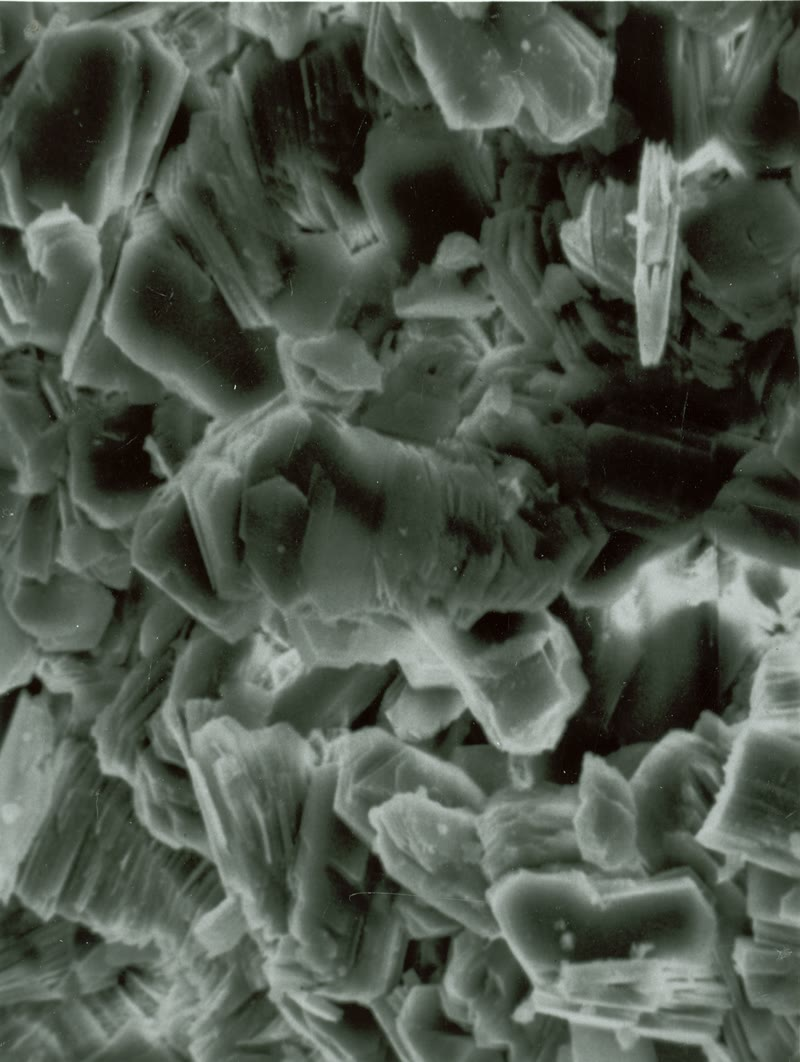
\includegraphics[width=\linewidth]{images/book3/b1-kaolinite-sem.jpg}

{\scriptsize \omterm{def:b1:weathering-clays:clay-mineral}{Kaoliniet} gezien met een rasterelektronenmicroscoop: boeken van gestapelde zeshoekige plaatjes, gegroeid in de poriën van een zandsteen uit het noorden van Alaska (vergroting ongeveer 1340). U.S. Geological Survey, publiek domein, via Wikimedia Commons.\par}
\end{minipage}
\end{omfigure}
% ledger: biscaye:1965, usgs:clay-settings, pedron:stages, commons:kaolinite-sem

\emph{\omterm{def:b1:weathering-clays:laterite}{Lateriet}.} Waar \omterm{def:b1:weathering-clays:hydrolysis}{hydrolyse} lang zijn laatste graden bereikt, wordt het profiel dikker en concentreert zijn top alles wat niet vertrekt.

\begin{definition}[Lateriet]\label{def:b1:weathering-clays:laterite}
Een \emph{lateriet}\index{lateriet} is het ijzer- en aluminiumrijke product van intense en langdurige \omterm{def:b1:weathering-clays:hydrolysis}{hydrolyse} onder hete, natte klimaten: een rood tot bruin materiaal, zacht of verhard, gemaakt van \omterm{def:b1:weathering-clays:clay-mineral}{kaoliniet} en ijzeroxiden en -hydroxiden, met gibbsiet waar \omterm{def:b1:weathering-clays:hydrolysis-degree}{allitisatie} is bereikt, waaruit bijna alle alkali- en aardalkalikationen en veel van het silicium zijn verwijderd.
\end{definition}
% ledger: formoso:laterite, buchanan:laterite

Een \omterm{def:b1:weathering-clays:laterite}{lateriet} die rijk genoeg is aan gibbsiet of boehmiet, de aluminiumhydroxiden, is een bauxiet, het erts van negen tiende van het aluminium: \omterm{def:b1:weathering-clays:hydrolysis-degree}{allitisatie} is de stap die het erts maakt. De meeste bauxieten zijn residueel, de rots waaruit alles behalve de aluminiumoxide is uitgeloogd; de meeste van die uit gibbsiet liggen in de tropen, en veel vormen zich waarschijnlijk nog.
% ledger: usgs:bauxite

\begin{history}[Een woord uit het veld]
In 1807 beschreef Francis Buchanan, die in Malabar in het zuiden van India reisde, een materiaal vol holten en rijk aan rode en gele ijzerokers, verspreid over het graniet in grote massa's. Uit de grond gegraven was het zo zacht dat een mes het sneed, en de bewoners vormden het tot blokken; in de lucht werd het al snel zo hard als baksteen, en het hield langer dan welke baksteen hij had gezien. De lokale talen noemden het baksteensteen; hij stelde de naam \omterm{def:b1:weathering-clays:laterite}{lateriet} voor, die de geologie hield voor de rode producten van tropische verwering.
\end{history}
% ledger: buchanan:laterite

\section{Silicaatverwering en koolstofdioxide}\label{sec:b1:weathering-clays:co2}

De waterstofionen van \omterm{def:b1:weathering-clays:hydrolysis}{hydrolyse} komen vooral van koolstofdioxide, dus door ze als koolzuur te schrijven, zien we wat verwering met de lucht doet. Voor een calciumsilicaat, voor de eenvoud geschreven als \ce{CaSiO3},
\[
  \ce{CaSiO3 + 2 CO2 + H2O -> Ca^2+ + 2 HCO3- + SiO2},
\]
en in de oceaan, waar organismen schelpen van calciumcarbonaat bouwen,
\[
  \ce{Ca^2+ + 2 HCO3- -> CaCO3 + CO2 + H2O}.
\]

\begin{proposition}[Verwering en koolstofdioxide]\label{prop:b1:weathering-clays:co2}
(a) Verwering van een silicaat verbruikt twee mol koolstofdioxide, omgezet tot bicarbonaat, voor elke mol vrijgekomen calcium of magnesium; wanneer het calcium of magnesium als carbonaat neerslaat, keert één van de twee terug naar de lucht, en wordt één mol als carbonaatgesteente opgeslagen. (b) Verwering van een carbonaatgesteente en het opnieuw neerslaan van zijn carbonaat slaat niets op.
\end{proposition}

\begin{proof}
(a) Het optellen van de twee vergelijkingen hierboven geeft \ce{CaSiO3 + CO2 -> CaCO3 + SiO2}: één \ce{CO2} per calcium verlaat de lucht voorgoed; de eerste vergelijking alleen toont de twee verbruikte. Voor magnesium geldt hetzelfde, met \ce{Mg^2+} voor \ce{Ca^2+}. (b) De oplossing van calciet, \ce{CaCO3 + CO2 + H2O -> Ca^2+ + 2
HCO3-}, is precies het omgekeerde van de neerslag: de som van de twee is nul.
\end{proof}

Met een \omterm{def:b1:rock-forming-minerals:groups}{veldspaat} vervangt het koolzuur de waterstofionen van \cref{prop:b1:weathering-clays:feldspars}: elke verbruikte \ce{H+} is één \ce{CO2} omgezet in \ce{HCO3-}. Het anorthiet van een basalt of een gabbro verbruikt zo twee mol koolstofdioxide per mol terwijl het in \omterm{def:b1:weathering-clays:clay-mineral}{kaoliniet} verandert,
\[
  \ce{CaAl2Si2O8 + 2 CO2 + 3 H2O -> Al2Si2O5(OH)4 + Ca^2+ + 2 HCO3-},
\]
en slaat er één op op de lange termijn. Natrium en kalium vormen op de zeebodem geen carbonaat, en de opslag op lange termijn wordt geteld uit het calcium en magnesium dat vrijkomt.

Rivieren voeren het bicarbonaat naar zee, en hun scheikunde meet de flux.
Uit de scheikunde van de grote rivieren van de wereld is geschat dat het koolstofdioxide dat door de verwering van continentale silicaten wordt verbruikt, \num{11.7e12} tot \qty{13.6e12}{mol} per jaar bedraagt, ongeveer 0.14 tot 0.16 miljard ton koolstof, waarvan alleen de verwering van basalten 30 tot \qty{35}{\percent} verklaart. De flux is klein naast de uitwisselingen van koolstof tussen de lucht, de oceanen en levende wezens, maar hij keert niet om: over miljoenen jaren is hij de belangrijkste weg waarlangs koolstofdioxide van vulkanen uit de atmosfeer verdwijnt. Omdat verwering sneller verloopt wanneer het warmer en natter is, bindt zij het koolstofdioxide van de lucht aan het klimaat, dat op zijn beurt van het koolstofdioxide afhangt via het broeikaseffect: een negatieve terugkoppeling die de temperatuur van de Aarde over geologische tijd stabiel houdt, bestudeerd in Boek~4.
% ledger: dessert:silicate-co2, whk:1981

\section{Oefeningen}

\begin{exercise}[$\star$]\label{exo:b1:weathering-clays:1}
Gebruik de stralen \ce{K+} \qty{1.38}{\angstrom}, \ce{Fe^2+} \qty{0.78}{\angstrom}, \ce{Fe^3+} \qty{0.645}{\angstrom} en \ce{Ti^4+} \qty{0.605}{\angstrom}: bereken de \omterm{def:b1:weathering-clays:ionic-potential}{ionische potentiaal} van elk ion en benoem zijn veld. Waarom verliest een bodem die onder water staat zijn ijzer, terwijl een goed gedraineerde het behoudt?
% ledger: shannon:radii-b19
\end{exercise}

\begin{exercise}[$\star$]\label{exo:b1:weathering-clays:2}
Vier kleifracties worden met röntgenstralen gemeten als georiënteerde preparaten. A: een piek bij \SI{14}{\angstrom}, verschoven naar \SI{17}{\angstrom} door ethyleenglycol en naar \SI{10}{\angstrom} door verhitting tot \SI{400}{\celsius}. B: een piek bij \SI{7}{\angstrom}, onveranderd door glycol, verdwenen na verhitting tot \SI{550}{\celsius}. C: een piek bij \SI{10}{\angstrom} die geen behandeling verplaatst. D: een piek bij \SI{14}{\angstrom} die geen behandeling verplaatst. Bepaal elk \omterm{def:b1:rock-forming-minerals:mineral}{mineraal}.
% ledger: usgs:clay-xrd
\end{exercise}

\begin{exercise}[$\star$]\label{exo:b1:weathering-clays:3}
Balanceer, met \cref{met:b1:weathering-clays:balance}, de \omterm{def:b1:weathering-clays:hydrolysis}{hydrolyse} van ortoklaas \ce{KAlSi3O8} tot \omterm{def:b1:weathering-clays:clay-mineral}{kaoliniet}, en bepaal welk deel van zijn kalium en van zijn silicium in oplossing verdwijnt.
\end{exercise}

\begin{exercise}[$\star$]\label{exo:b1:weathering-clays:4}
(a) Bereken het volume ijs dat \qty{10}{cm^3} water bij \qty{0}{\celsius} geeft. (b) Bepaal binnen welk temperatuurbereik ijs dat in scheuren groeit de rots het meest doeltreffend splijt, en leg uit waarom noch een lichtere noch een strengere vorst even goed doet. (c) Een kubus graniet met zijde \qty{1}{m} wordt door vorst gesplitst in kubusjes met zijde \qty{1}{cm}: bereken met welke factor haar oppervlak is toegenomen.
% ledger: usgs:water-density, iapws:ice-density, wh85:frost
\end{exercise}

\begin{exercise}[$\star\star$]\label{exo:b1:weathering-clays:5}
Bereken het specifieke oppervlak van veldspaatkorrels met dichtheid \qty{2600}{kg.m^{-3}}, als kubusjes beschouwd, voor afmetingen van \qty{1}{cm}, \qty{1}{mm} en \qty{1}{\micro m}. Leg uit waarom de korrelgrootte zo sterk van belang is voor de snelheid van \omterm{def:b1:weathering-clays:weathering}{chemische verwering}, en waarom \omterm{def:b1:weathering-clays:weathering}{fysische verwering} \omterm{def:b1:weathering-clays:weathering}{chemische verwering} versnelt.
\end{exercise}

\begin{exercise}[$\star\star$]\label{exo:b1:weathering-clays:6}
Een ton albiet \ce{NaAlSi3O8} (\qty{262.22}{g.mol^{-1}}) wordt omgezet in \omterm{def:b1:weathering-clays:clay-mineral}{kaoliniet} (\qty{258.16}{g.mol^{-1}}). Bereken de massa van gevormd \omterm{def:b1:weathering-clays:clay-mineral}{kaoliniet}, de massa van het uitgevoerde silica, geteld als \ce{SiO2} (\qty{60.08}{g.mol^{-1}}), en de massa van het uitgevoerde natrium.
% ledger: webmineral:clays-b19, ciaaw:Na
\end{exercise}

\begin{exercise}[$\star\star$]\label{exo:b1:weathering-clays:7}
Een graniet bevat, naar massa, \qty{0.30}{\percent} \ce{TiO2}, \qty{3.5}{\percent} \ce{Na2O}, \qty{72}{\percent} \ce{SiO2} en \qty{14}{\percent} \ce{Al2O3}; zijn saproliet bevat \qty{0.60}{\percent} \ce{TiO2}, \qty{0.35}{\percent} \ce{Na2O}, \qty{60}{\percent} \ce{SiO2} en \qty{27}{\percent} \ce{Al2O3}. Neem titaan als onbeweeglijk aan, en bepaal de massa saproliet die een kilogram graniet achterlaat, het deel van het natrium, het silicium en het aluminium dat verloren gaat, en welke graad van \omterm{def:b1:weathering-clays:hydrolysis}{hydrolyse} aan de gang is.
\end{exercise}

\begin{exercise}[$\star\star$]\label{exo:b1:weathering-clays:8}
Gebruik \cref{prop:b1:weathering-clays:layer-charge} en bereken de laaglading van pyrofylliet \ce{Al2Si4O10(OH)2}, van muscoviet \ce{KAl2(Si3Al)O10(OH)2} zonder zijn kalium, van de beidellietlaag \ce{Al2(Si_{3.5}Al_{0.5})O10(OH)2} en van een montmorilloniet-laag \ce{(Al_{1.67}Mg_{0.33})Si4O10(OH)2}. Bepaal welke ervan kunnen zwellen, en leg uit waarom.
% ledger: webmineral:clays-b19
\end{exercise}

\begin{exercise}[$\star\star$]\label{exo:b1:weathering-clays:9}
Forsteriet \ce{Mg2SiO4} verweert volgens
\ce{Mg2SiO4 + 4 CO2 + 4 H2O -> 2 Mg^2+ + 4 HCO3- + H4SiO4}. (a) Controleer de
vergelijking. (b) Bereken voor een ton forsteriet het verbruikte koolstofdioxide en
het op lange termijn opgeslagen koolstofdioxide volgens
\cref{prop:b1:weathering-clays:co2}. (c) Bepaal wat dezelfde berekening geeft voor een ton calciet.
% ledger: ciaaw:Mg, ciaaw:Si, ciaaw:O, ciaaw:C
\end{exercise}

\begin{exercise}[$\star\star\star$]\label{exo:b1:weathering-clays:10}
(a) Bepaal tussen welke stralen een ion met lading 3 een hydrolysaat is. (b) Bepaal in welke vorm boor, \ce{B^3+}, met een straal van \qty{0.27}{\angstrom}, in water reist. (c) \ce{Mn^2+} heeft een straal van \qty{0.83}{\angstrom}, \ce{Mn^4+} van \qty{0.53}{\angstrom}. Leg uit waarom zwarte \omterm{def:b1:layered-earth:layers}{korsten} van mangaanoxide ontstaan waar bronwater, arm aan zuurstof, de lucht in komt. (d) Leg uit waarom silicium noch volledig kan worden uitgeloogd, noch volledig behouden blijft.
% ledger: shannon:radii-b19, nomad:goldschmidt
\end{exercise}

\begin{exercise}[$\star\star\star$]\label{exo:b1:weathering-clays:11}
De verwering van continentale silicaten verbruikt \num{11.7e12} tot \qty{13.6e12}{mol} koolstofdioxide per jaar, waarvan \qty{4.08e12}{mol} uit basalten. (a) Reken het bereik om naar ton koolstof en koolstofdioxide per jaar. (b) Welk aandeel nemen de basalten? (c) Als dit alles uit calcium- en magnesiumsilicaten kwam, hoeveel koolstof zou dan elk jaar op lange termijn worden opgeslagen? Leg uit waarom het werkelijke lange-termijncijfer kleiner is.
% ledger: dessert:silicate-co2, ciaaw:C, ciaaw:O
\end{exercise}

\begin{exercise}[$\star\star\star$]\label{exo:b1:weathering-clays:12}
Drie kleifracties, bevrijd van kwarts en ijzeroxiden, worden geanalyseerd (massaprocent): A, \ce{SiO2} \num{46.55} en \ce{Al2O3} \num{39.50}; B, \ce{SiO2} 60 en \ce{Al2O3} 25; C, \ce{SiO2} 2 en \ce{Al2O3} 63 (\ce{SiO2} \qty{60.08}{g.mol^{-1}}, \ce{Al2O3} \qty{101.96}{g.mol^{-1}}). Bereken de molaire verhouding Si/Al van elk, bepaal welke graad van \omterm{def:b1:weathering-clays:hydrolysis}{hydrolyse} zij registreert, en plaats de drie bodems op een lijn van de minst naar de intensiefste uitloging.
% ledger: webmineral:clays-b19, pedron:stages, formoso:laterite
\end{exercise}

\section{Probleem: van graniet naar klei}

\begin{problem}[{Weekendprobleem --- de veldspaten van een graniet en een gabbro, van de gebalanceerde reacties tot het koolstofdioxide dat een rivier wegvoert}]
\label{pb:b1:weathering-clays:1}
% values: calc/ch19.py; the river is invented (its numbers are of a realistic order)
De veldspaten zijn albiet \ce{NaAlSi3O8} (\qty{262.22}{g.mol^{-1}}, dichtheid \qty{2.62}{g.cm^{-3}}) en anorthiet \ce{CaAl2Si2O8} (\qty{278.20}{g.mol^{-1}}, dichtheid \qty{2.75}{g.cm^{-3}}). \omterm{def:b1:weathering-clays:clay-mineral}{Kaoliniet} \ce{Al2Si2O5(OH)4} heeft de molaire massa \qty{258.16}{g.mol^{-1}} en de dichtheid \qty{2.6}{g.cm^{-3}}; gibbsiet \ce{Al(OH)3}, \qty{78.00}{g.mol^{-1}}. Neem \ce{SiO2} \qty{60.08}{g.mol^{-1}}, \ce{CO2} \qty{44.01}{g.mol^{-1}}, \ce{HCO3-} \qty{61.02}{g.mol^{-1}}, Na \num{22.99} en Ca \qty{40.08}{g.mol^{-1}}.
% ledger: hom:albite, hom:anorthite, webmineral:clays-b19, ciaaw:Na, ciaaw:Ca, ciaaw:C, ciaaw:O, ciaaw:H

\medskip
\noindent\textbf{Deel I --- De reacties.}
\begin{enumerate}
  \item Balanceer de \omterm{def:b1:weathering-clays:hydrolysis}{hydrolyse} van albiet tot \omterm{def:b1:weathering-clays:clay-mineral}{kaoliniet}.
  \item Balanceer de \omterm{def:b1:weathering-clays:hydrolysis}{hydrolyse} van anorthiet tot \omterm{def:b1:weathering-clays:clay-mineral}{kaoliniet}, en leg uit wat er bijzonder aan is.
  \item Balanceer de \omterm{def:b1:weathering-clays:hydrolysis}{hydrolyse} van anorthiet tot gibbsiet.
  \item Balanceer de \omterm{def:b1:weathering-clays:hydrolysis}{hydrolyse} van albiet tot beidelliet \ce{Na_{0.5}Al2(Si_{3.5}Al_{0.5})O10(OH)2}, en controleer het waterstof.
  \item Herschrijf de eerste twee reacties met koolzuur als bron van de waterstofionen: \ce{CO2 + H2O -> H+ + HCO3-}.
  \item Bepaal welke van deze reacties \omterm{def:b1:weathering-clays:hydrolysis-degree}{bisiallitisatie}, \omterm{def:b1:weathering-clays:hydrolysis-degree}{monosiallitisatie} en \omterm{def:b1:weathering-clays:hydrolysis-degree}{allitisatie} zijn.
\end{enumerate}

\medskip
\noindent\textbf{Deel II --- Wat blijft, wat vertrekt.}
\begin{enumerate}[resume]
  \item Bereken hoeveel mol er zit in een ton albiet, en in een ton anorthiet.
  \item Bereken de massa \omterm{def:b1:weathering-clays:clay-mineral}{kaoliniet} die uit een ton van elk wordt gevormd.
  \item Bereken de massa's silica (als \ce{SiO2}), natrium en calcium die in oplossing worden uitgevoerd.
  \item Bereken het volume van een ton van elk \omterm{def:b1:rock-forming-minerals:groups}{veldspaat} en van het \omterm{def:b1:weathering-clays:clay-mineral}{kaoliniet} dat het geeft, en bepaal met welk deel het volume van het vaste stof krimpt.
  \item Geef aan wat de ruimte vult die is achtergebleven in een verweerd graniet rijk aan albiet, en leg uit waarom een verweerde gabbro rijk aan anorthiet dichter blijft.
  \item Leg met het ionische-potentiaaldiagram uit welke van de elementen van de twee veldspaten vertrekken en welke blijven.
\end{enumerate}

\medskip
\noindent\textbf{Deel III --- Koolstofdioxide.}
\begin{enumerate}[resume]
  \item Bereken hoeveel mol en hoeveel kilogram koolstofdioxide wordt verbruikt wanneer een ton albiet in \omterm{def:b1:weathering-clays:clay-mineral}{kaoliniet} verandert.
  \item Beantwoord dezelfde vraag voor een ton anorthiet.
  \item Bereken welke massa bicarbonaat het anorthiet uitvoert.
  \item Beschrijf wat er met dit bicarbonaat in de oceaan gebeurt, en bepaal hoeveel van het verbruikte koolstofdioxide naar de lucht terugkeert.
  \item Leg uit waarom er geen opslag op lange termijn wordt geteld voor het natrium van de albiet.
  \item Vergelijk dit met de oplossing van een ton calciet, gevolgd door zijn neerslag.
\end{enumerate}

\medskip
\noindent\textbf{Deel IV --- Een rivier.}
\begin{enumerate}[resume]
  \item Een rivier voert \qty{50000}{km^2} graniet en gneis af, met een gemiddelde afvoer van \qty{200}{m^3.s^{-1}}; het bicarbonaat dat zij uit silicaatverwering meevoert, is \qty{0.3}{mmol.L^{-1}}. Bereken de jaarlijkse flux van dit bicarbonaat, in mol, en per vierkante kilometer.
  \item Druk die uit als de mol anorthiet waarvan de verwering tot \omterm{def:b1:weathering-clays:clay-mineral}{kaoliniet} het zou leveren, en vervolgens als ton anorthiet per jaar en per vierkante kilometer.
  \item Als het gesteente het equivalent van \qty{20}{\percent} anorthiet bevat en de dichtheid \qty{2700}{kg.m^{-3}} heeft, bereken dan met welke snelheid, in meter per miljoen jaar, het verse gesteente wordt verbruikt.
  \item Hoeveel koolstofdioxide haalt deze rivier elk jaar voorgoed uit de lucht?
  \item Leg uit waarom de snelheid van vraag 21 een ondergrens is voor de daling van het landoppervlak.
  \item Bereken, in kilogram op drie cijfers nauwkeurig, hoeveel koolstofdioxide voorgoed wordt onttrokken door de verwering van één ton anorthiet.
\end{enumerate}
\end{problem}
